\documentclass[11pt]{article}
\usepackage[margin=1in]{geometry}
\usepackage{amsmath,amssymb}
\usepackage{booktabs}
\usepackage{graphicx}
\usepackage{caption}
\usepackage{siunitx}
\usepackage{url}
\usepackage{enumitem}
\usepackage{xcolor}
\usepackage[colorlinks=true,linkcolor=black,citecolor=blue,urlcolor=blue]{hyperref}

\graphicspath{{figures/}}
\newcommand{\ppl}{\ensuremath{\times}}
\emergencystretch=2.2em

\title{\textbf{Zero-Miss or Nothing: The Concurrency Boundary of\\
Mixture-of-Experts Serving on Apple Silicon}}
\author{Youssef Hariri\\
DeeWaanAI (Mug and Bewong Ltd)\\
\texttt{youssef.hariri@rennes-sb.com}\\
\texttt{ORCID 0009-0009-5374-586X}}
\date{Preprint --- November 2026\\ \small DOI: 10.5281/zenodo.24466028}

\begin{document}
\maketitle

\begin{abstract}
\noindent
A 2025--26 wave of systems made single-user Mixture-of-Experts (MoE)
inference fast on consumer hardware through dynamic expert caches,
predictive prefetch, SSD streaming, and trained routing predictors. These
systems are evaluated almost exclusively with a single user and a mean
throughput metric. We study how these mechanisms behave under the conditions
a local service actually faces: several concurrent users and a per-user tail
service-level objective, namely the 5th-percentile (p05) per-user decode
throughput against a \SI{10}{tok/s} floor --- the speed below which
interactive reading stalls --- measured on Apple-Silicon unified memory. We
port the field's mechanisms into an output-exact MLX engine (token-exact
routing, no retraining) and evaluate them on three models spanning a
$3.8\ppl$ to $0.9\ppl$ RAM-to-model ratio, plus a 235B-parameter frontier
model $8\ppl$ larger than the machine. Single-user, the ports work: an LRU
expert cache beats static pinning by $43\%$ at $75\%$ capacity and
double-buffered prefill is $2.1$--$2.6\ppl$ faster, all token-exact.
Under concurrency the picture inverts: every partial-residency configuration
--- LRU at any capacity, a hybrid pin-and-cache, mmap tiering --- collapses
below the floor by four users, while only a \emph{zero-miss} configuration
(full static residency) protects the tail (12 users on OLMoE-1B-7B). The
law follows: under a tail metric, expert residency is all-or-nothing,
because one miss costs ${\sim}100\ppl$ a hit and the p05 user is by
construction the one who experiences it. It holds across all three models
and is invisible to the single-user literature, whose systems are
single-request by design. Two further results: on Edge0's own engine, exact
routing costs $1.7\ppl$ single-user speed (12.45 vs 21.07 tok/s); and our
engine serves a 235B model on a 16\,GB laptop exactly, at $0.103$ tok/s.
Every number traces to a frozen artifact, with run-to-run variance reported
per cell.
\medskip
\noindent\textbf{Keywords:} mixture-of-experts; edge inference; Apple
Silicon; unified memory; expert caching; tail latency; multi-tenant
serving; p05 SLO
\end{abstract}
\newpage

\section{Introduction}

Two years of systems work have made large MoE models \emph{individually}
usable on consumer hardware. FreeToken~\cite{freetoken} serves 284B-class
models on a gaming PC with a global LRU expert cache, double-buffered
prefill, and bandwidth-adaptive CPU--GPU co-execution. Edge0~\cite{edge0}
streams a 35B model from SSD on a 24\,GB Mac mini at 20\,tok/s inside
3\,GiB of active memory, using a trained prerouter that replaces the model's
routing one token ahead. Open releases such as SlotStream~\cite{slotstream}
and SwiftLM~\cite{swiftlm} stream 100B+ models to MacBooks. A user with a
laptop can, today, talk to a frontier model --- alone.

Almost none of this work is evaluated the way a local model is actually
\emph{used}: shared. A personal assistant, a household server, or a small
team's on-premise endpoint serves several concurrent sessions, and what
matters to each user is not the mean but the tail --- the slowest experience
anyone gets. Prior work by the author measured exactly this with a p05
concurrency ceiling on Apple Silicon and found that static expert pinning
pays only when the model is a small fraction of RAM~\cite{hariri2026pinning}.
That study predated the 2026 cache wave, and the obvious question followed:
do the new mechanisms change the answer?

This paper ports the wave's mechanisms into an output-exact engine and
measures them under the tail. The answer is a law, and it is not kind to
the wave.

\paragraph{Contributions.}
\begin{enumerate}[leftmargin=1.7em,itemsep=1pt,topsep=3pt]
  \item \textbf{Mechanism transfer, measured} (Section~\ref{sec:transfer}):
        LRU expert caching ($+43\%$ single-user at $75\%$ capacity),
        double-buffered prefill ($2.1$--$2.6\ppl$), mmap kernel tiering
        (a negative result), and a predictability ceiling for training-free
        routing oracles ($0.465$ recall) --- all token-exact, all on unified
        memory.
  \item \textbf{The two-class law} (Section~\ref{sec:law}): under a per-user
        p05 SLO, every partial-residency configuration --- LRU at four
        capacities, a hybrid pin-and-cache design, mmap tiering ---
        collapses with concurrency, while zero-miss full residency holds 12
        users on the model that fits.
  \item \textbf{The price of exactness} (Section~\ref{sec:exactness}): on
        Edge0's own engine, its two routing modes differ by $1.7\ppl$
        single-user speed (12.45 exact vs 21.07 predicted tok/s), an
        independent reproduction of their central claim under our protocol.
  \item \textbf{A frontier feasibility point}
        (Section~\ref{sec:frontier}): an exact, unmodified 235B-A22B model
        served on a 16\,GB laptop at $0.103$ tok/s with a 9\,GB peak memory
        footprint, reported with concurrency context.
  \item \textbf{Variance as evidence} (Section~\ref{sec:law}): dynamic
        caches exhibit markedly wider run-to-run spread than static
        configurations under load --- they are less predictable, not merely
        slower.
\end{enumerate}

\paragraph{Scope and non-claims.} We do not claim the fastest engine;
Edge0's C++ implementation outperforms our Python/MLX path per byte
(Section~\ref{sec:exactness}), and we report that gap openly. We do not
claim batching-optimal ceilings: our concurrency protocol time-slices rather
than batches, so all ceilings are conservative lower bounds
(Section~\ref{sec:method}). We do not evaluate FreeToken's $q^\star$
CPU--GPU miss splitting, which has no meaning where CPU and GPU share one
physical memory pool; we note this as an architectural observation rather
than an experiment.

\section{Related Work}
\label{sec:related}

\paragraph{Expert offloading and caching.}
Serving MoE models whose expert pool exceeds device memory has converged on
a common architecture: the complete pool resides in host memory or on disk
and a subset is cached for compute. EdgeMoE established the pattern
on-device~\cite{edgemoe}; Mixtral-offloading combined an LRU expert cache
with speculative prefetching~\cite{mixtraloffloading}; MoE-Infinity traced
request-level activation patterns to guide caching~\cite{moeinfinity};
ProMoE, ExpertFlow, and FineMoE sharpened the predictors that anticipate
routing~\cite{promoe,expertflow,finemoe}. Fine-grained offloading analyses
target the latency--memory trade-off directly~\cite{finemoe}. SliceMoE
caches experts at slice granularity with mixed precision, and MoE-CORE
allocates cache budgets layer-wise~\cite{slicemoe,moecore}. Diff-MoE
exploits layer-specific locality~\cite{diffmoe}. All of these systems are
evaluated with a single user and a mean metric; none reports a tail
concurrency ceiling.

\paragraph{Prediction and prefetch.}
A parallel line predicts future routing: ProMoE and
FineMoE~\cite{promoe,finemoe} from intermediate states, SP-MoE and
MoE-SpeQ co-design speculative decoding with expert
prefetch~\cite{spmoe,moespeq}, and PROBE balances prediction against
communication in real time~\cite{probe}. Our own prior measurement found
training-free predictive prefetch counterproductive on single-SSD consumer
hardware~\cite{hariri2026pinning}; Edge0's trained prerouter is the
output-changing exception we price in Section~\ref{sec:exactness} rather
than adopt. Yu et al.\ show prefetching can harm under contention by
interleaving concurrent requests~\cite{interleaving} --- the closest prior
observation to our concurrency finding, though still without a tail metric.

\paragraph{Streaming from SSD on Apple Silicon.}
Edge0~\cite{edge0}, SlotStream~\cite{slotstream}, and
SwiftLM~\cite{swiftlm} stream 35B--125B models from NVMe on Macs at
5--20 tok/s single-user. All are single-request engines; none reports
concurrent behavior. Our frontier point (Section~\ref{sec:frontier}) extends
this regime to 235B with exactness and memory accounting.

\paragraph{Cache ownership and approximation.}
``Who Should Own the Expert Cache?'' argues for kernel-managed
tiering~\cite{kernelcache}; our mmap arm tests that position on unified
memory and reports a negative (Section~\ref{sec:transfer}). OD-MoE removes
the cache entirely in favor of on-demand loading~\cite{odmoe}. HOBBIT,
PagedMoE, and GEMQ reduce miss cost by serving low-precision expert
replicas~\cite{hobbit,pagedmoe,gemq}; these change outputs and are excluded
from our default configurations by the exactness contract. Cache-aware
routing retrains or constrains the router toward resident
experts~\cite{cecar,psrouting,cacheaware} and is excluded for the same
reason. The qs inequality formalizes the KV--expert contention we observe
empirically~\cite{qsineq}.

\paragraph{Tail-latency measurement.}
FairBatching, Niyama, and SLO-aware sliding-window scheduling motivate
low-percentile service metrics over means~\cite{fairbatching,niyama,slosw}.
Roofline analyses caution that batch-1 decode is memory-bound but not purely
bandwidth-limited~\cite{memnotbw}; we therefore compare engines to each
other rather than to theoretical peaks.

\paragraph{Prior work by the author.}
\emph{When Pinning Pays}~\cite{hariri2026pinning} measured pinned-expert
orchestration against llama.cpp on Apple Silicon, reporting a
ratio-conditional concurrency crossover (a $2\ppl$ win at a $3.8\ppl$
RAM-to-model ratio, vanishing below ${\sim}2\ppl$), a $>$RAM feasibility
result, and disciplined negatives on predictive prefetch and
residency-for-KV eviction. The present work treats that study's engine as
the baseline and asks whether the 2026 mechanism wave escapes its boundary.
Where the two protocols differ, we reconcile in
Section~\ref{sec:reconciliation}.

\section{System, Metric, and Method}
\label{sec:method}

\paragraph{The exactness contract.}
The served model must answer as the original model: token-exact output, the
native router authoritative, no retraining, no quality-recovery adapters.
All mechanisms we adopt are systems-only: they change \emph{when} and
\emph{where} expert bytes reside, never \emph{what} is computed.
Output-changing mechanisms (predicted routing, low-bit replicas) appear
only as labeled arms (Section~\ref{sec:exactness}). Parity with the stock
model is verified per configuration; the single residual divergence class
is a measured near-tie (top-2 logit margin $0.078$), consistent with the
near-tie rounding behavior disclosed in prior work~\cite{hariri2026pinning}.

\paragraph{Engine configurations.}
All configurations share a stock \texttt{mlx\_lm} backbone with only the MoE
block replaced: (i)~\emph{static} --- a traffic-ranked pinned expert set
with a gather-QMM fast path~\cite{hariri2026pinning}; (ii)~\emph{LRU} --- a
per-layer pool of fixed slots with sticky-slot in-place updates and
least-recently-used eviction that never evicts an expert required by the
current step; prefill working sets larger than the pool are served
exact-but-uncached (an in-step eviction bug caught during development would
otherwise corrupt the step); (iii)~\emph{hybrid} --- a calibrated hot set
pinned into protected slots, the remainder LRU-managed; (iv)~\emph{mmap}
--- no explicit cache, with MLX's mmap-backed lazy loader and the kernel
page cache as the only tier. A double-buffered prefill streamer, hard-capped
at 16 in-flight reads, overlaps next-layer slab reads with current-layer
compute.

\paragraph{Metric and protocol.}
The primary metric is the p05 concurrency ceiling: the largest number of
simultaneous users $N$ for which the 5th-percentile per-user decode
throughput remains at or above \SI{10}{tok/s}. We use distinct frozen
WildChat prompts per user, 100-token generations, three repetitions per
cell, and report medians with per-cell spread. Concurrency is realized as
round-robin time-slicing on one engine instance, with per-user rate computed
as tokens divided by wall-clock from decode-phase start to that user's
completion. Time-slicing understates the throughput of a batched server;
ceilings are therefore conservative lower bounds, and the law of
Section~\ref{sec:law} is an ordering result that does not depend on the
batching model (Section~\ref{sec:reconciliation}). Every experimental unit
runs in its own OS process (a memory-isolation lesson learned through two
incidents, Appendix~B).

\paragraph{Hardware.}
A 16\,GB M1 Pro MacBook Pro with a single internal SSD. All configurations
share the machine, the prompts, and 4-bit group-64 quantization.

\section{Mechanism Transfer: What Survives Without a PCIe Bus}
\label{sec:transfer}

\subsection{Single-user results (OLMoE-1B-7B, equal memory budgets)}

\begin{figure}[t]
\centering
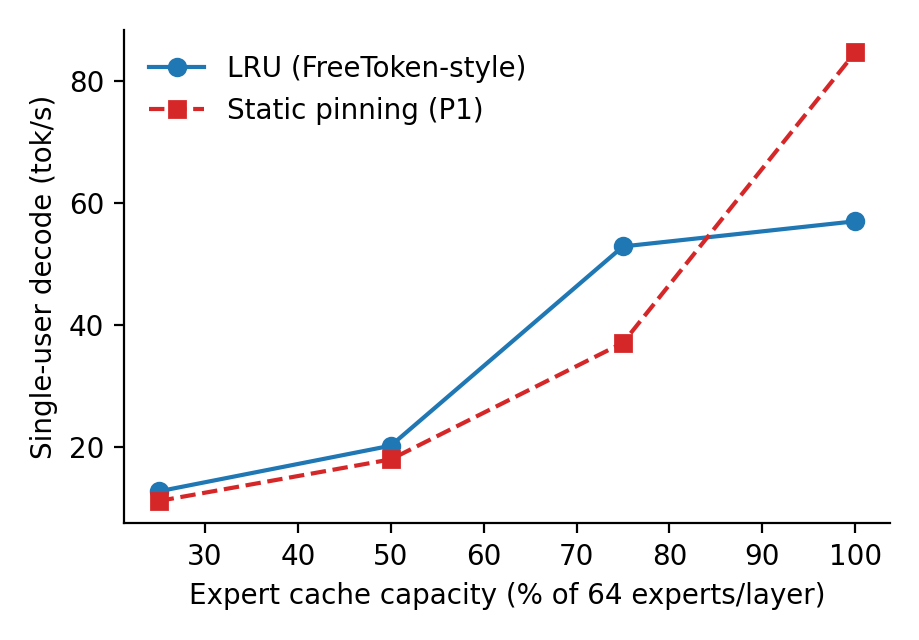
\includegraphics[width=0.62\linewidth]{figA_capacity_sweep.png}
\caption{Single-user decode versus expert-cache capacity (OLMoE, equal
budget, median over 3 prompts). Dynamic LRU wins the mid-band; static's
zero-sync fast path wins at full residency.}
\label{fig:capacity}
\end{figure}

\begin{table}[h]
\centering
\caption{Single-user decode on OLMoE-0125 (16\,GB M1 Pro, median over 3
prompts). Static $=$ traffic-ranked pinning; LRU $=$ ported FreeToken-style
cache.}
\label{tab:transfer}
\small
\begin{tabular}{lccc}
\toprule
Capacity (of 64 experts) & Static & LRU & Winner \\
\midrule
16 (25\%)  & 11.2 & 12.8 & tie \\
32 (50\%)  & 18.0 & 20.3 & tie \\
48 (75\%)  & 37.1 & \textbf{52.9} & LRU $+43\%$ \\
64 (100\%) & \textbf{84.8} & 57.1 & static (zero-sync fast path) \\
\bottomrule
\end{tabular}
\end{table}

Double-buffered prefill yields $2.63\ppl/2.31\ppl$ (256-token prompts) and
$2.18\ppl/2.13\ppl$ (512-token) prefill speedups with decode unchanged and
output exact. The mmap kernel tier reaches $5.7$ tok/s --- $2.2\ppl$ slower
than LRU at $25\%$ capacity and $9\ppl$ slower at $75\%$ --- because the
kernel reclaims the working set aggressively and per-expert dispatch
dominates; we report this as a careful negative against the datacenter
finding of~\cite{kernelcache}. Training-free routing prediction on
Qwen3-30B shows temporal recall $0.465$ against a popularity baseline of
$0.371$: real structure, but below the threshold prior measurement showed
profitable on single-SSD hardware~\cite{hariri2026pinning}; the oracle was
accordingly not built (a bounded pre-negative).

\paragraph{Design rule.}
\emph{Pin when the model fits, cache when it does not, double-buffer
always.} The single-user literature could have produced this rule; it did
not, because it never swept capacity at equal budget.

\section{The Two-Class Law}
\label{sec:law}

\subsection{Crossover under concurrency}

\begin{figure}[t]
\centering
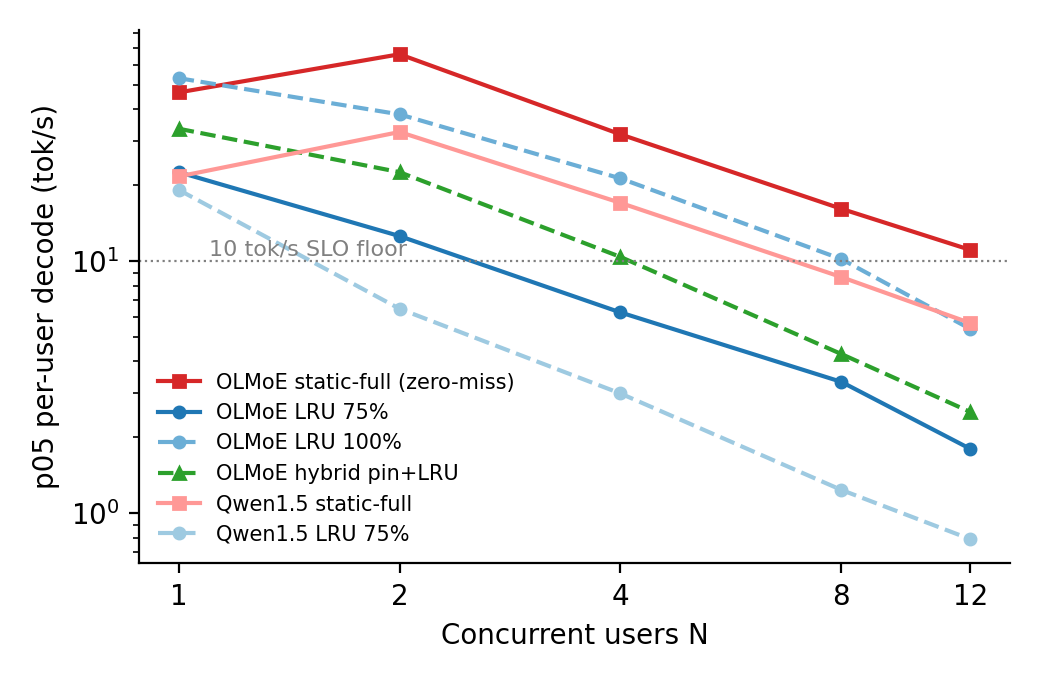
\includegraphics[width=0.78\linewidth]{figB_two_class_law.png}
\caption{The two-class law (medians of 3 runs, log--log). Zero-miss
configurations (red/pink) decay gently; every partial-residency
configuration dives through the 10 tok/s floor by $N{=}4$. The hybrid
inherits the cache class, not the static class. Ceilings are conservative
under the time-sliced protocol (Section~\ref{sec:method}).}
\label{fig:law}
\end{figure}

\begin{table}[h]
\centering
\caption{p05 per-user decode tok/s versus concurrent users (median of 3,
10 tok/s floor). Static-full is zero-miss by construction. Qwen3-30B has no
zero-miss configuration: 18\,GB $>$ 16\,GB.}
\label{tab:law}
\small
\begin{tabular}{lcccccc}
\toprule
Configuration & $N{=}1$ & $N{=}2$ & $N{=}4$ & $N{=}8$ & $N{=}12$ & Ceiling \\
\midrule
OLMoE static-full & 46.6 & 66.1 & 31.8 & 16.1 & 11.1 & \textbf{12} \\
OLMoE LRU (75\%)  & 22.5 & 12.6 & 6.3 & 3.3 & 1.8 & 2 \\
OLMoE LRU (100\%) & 30.2 & 21.6 & 10.9 & 5.4 & 3.6 & 4 \\
OLMoE hybrid      & 21.5 & 13.9 & 6.9 & 3.0 & 1.8 & 2 \\
Qwen1.5 static-full & 21.7 & 32.5 & 17.0 & 8.6 & 5.7 & \textbf{4} \\
Qwen1.5 LRU (75\%)  & 19.2 & 6.5 & 3.0 & 1.2 & 0.8 & 1 \\
Qwen3-30B LRU (50\%) & 7.9 & 5.1 & 1.6 & 0.9 & --- & 0 \\
\bottomrule
\end{tabular}
\end{table}

\subsection{The mechanism}

The pattern admits no middle case. A cache hit reads from RAM; a miss reads
from SSD at ${\sim}100\ppl$ the latency. Under a \emph{mean} metric, a $2\%$
miss rate costs little; under a \emph{tail} metric, the p05 user is by
construction the request whose steps absorb the misses. Concurrency worsens
this in two ways: the batch working set grows with users (measured in prior
work as $36\to56$ of 64 experts for 95\% batch
coverage~\cite{hariri2026pinning}), so every partial cache thrashes harder
as $N$ rises; and miss latency lands exactly on the slowest requests. Hence
the law:

\begin{quote}
\emph{Under a tail SLO, expert residency is all-or-nothing: configurations
with any misses collapse with concurrency; only a zero-miss configuration
protects the tail.}
\end{quote}

Corollaries, each measured: enlarging the cache does not fix it (LRU at
100\% capacity still loses, ceiling 4 vs 12); hybrid pinning inherits the
cache's thrash rather than the static configuration's robustness (refuted
at ceiling 2); and dynamic caches are \emph{far less predictable}, with
run-to-run spread of 46--105\% across nearly all cells versus 1--10\% for
static configurations away from the memory-pressure boundary (static low-$N$
cells on the 8.8\,GB model show 72--179\% pressure variance, disclosed in
Appendix~A). Variance compounds the tail penalty and is itself a tail
property. The ratio crossover of~\cite{hariri2026pinning} composes with the
law: zero-miss is affordable only when the model is a small enough fraction
of RAM (static ceiling 12 at $3.8\ppl$, 4 at $1.8\ppl$), so the regimes
partition cleanly --- \emph{zero-miss wins where it fits; everywhere else is
the feasibility regime}.

\subsection{Reconciliation with prior measurements}
\label{sec:reconciliation}
Our static OLMoE ceiling here is 12 versus 16 reported
in~\cite{hariri2026pinning}. We isolated the factors: prompt distribution
is not one (repeating the earlier shared-prompt protocol reproduces 12);
the residual is this study's round-robin time-slicing versus the earlier
work's true continuous batching, which understates ceilings conservatively.
The law is an ordering over configurations measured on a single protocol;
its direction is protocol-independent.

\section{The Price of Exactness}
\label{sec:exactness}

Edge0's engine offers two routing modes: \texttt{actual} (the model's
original computation) and \texttt{predicted} (the trained prerouter's).
Under our harness --- 16\,GB M1 Pro, a WildChat prompt, greedy decoding,
median of 3 fresh processes, the authors' own \texttt{bench} tool and
verified assets --- we measure \textbf{12.45 tok/s (actual) versus 21.07
tok/s (predicted)}: a $1.7\ppl$ single-user speed price for exact routing.
This independently reproduces their $+80$--$84\%$ claim at $+69\%$ on our
hardware, with sub-$0.3\%$ run spread. The quality cost is reported in their
paper ($-3.9$ mean benchmark points, $-6$ to $-10$ on long-chain
reasoning); our contract declines it. The framing this gives the present
work is direct: the $1.7\ppl$ is real, and it buys exactly \emph{one} user;
per Section~\ref{sec:law} it buys nothing against the tail at $N{>}1$, and
their engine is single-request by design. We also note openly that Edge0's
C++ path is faster per byte than our Python/MLX path (their exact-mode 12.45
tok/s versus our 7.9 tok/s on the comparable Qwen3-30B); the contribution
here is the measurement and the law, not the fastest binary.

\begin{figure}[t]
\centering
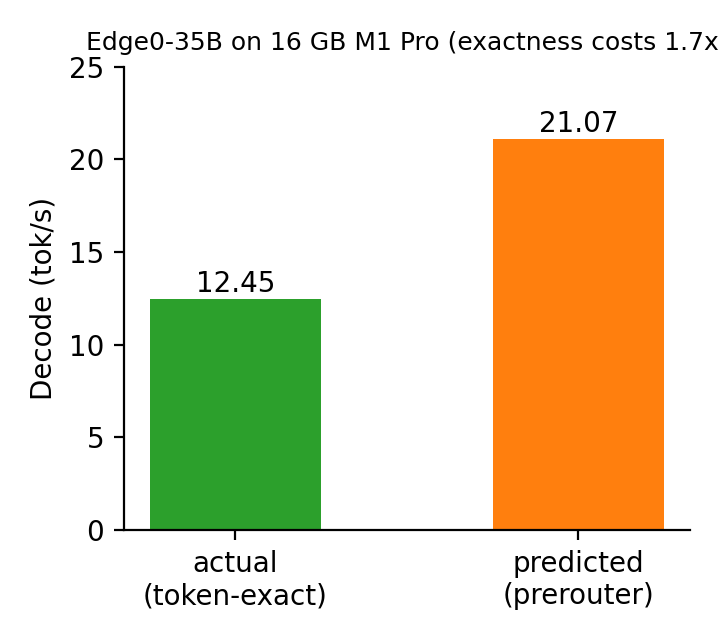
\includegraphics[width=0.5\linewidth]{figC_price_of_exactness.png}
\caption{The price of exactness on Edge0's own engine (median of 3, our
harness): predicted routing is $1.7\ppl$ faster --- and buys one user.}
\label{fig:exactness}
\end{figure}

\section{Frontier: 235B on a 16 GB Laptop}
\label{sec:frontier}

Qwen3-235B-A22B (130\,GB at 4-bit, 22B active) served by our engine (LRU,
4 slots per layer, streamer, lazy loading, 10\,GB cap): model load
$0.5$\,s, prefill $27.9$\,s, decode $0.103$ tok/s, $9.0$\,GB peak memory,
coherent output (Appendix~A). This is a feasibility result, not a speed
result: ${\sim}100\ppl$ below the SLO floor, with a p05 ceiling of 0 (the
single-user rate is already below the floor; a second user would document
nothing, so it is stated rather than run). The run followed an earlier smoke
test, so SSD pages were partially warm; a cold-cache figure would be slower
and is disclosed as such. To our knowledge this is the first 235B-on-16\,GB
measurement reported with exactness and concurrency context: the model
runs, exactly, for exactly one user.

\section{Threats to Validity}
\label{sec:threats}

\paragraph{Internal.} Round-robin time-slicing understates ceilings
(conservative direction; Section~\ref{sec:reconciliation}). LRU-versus-static
differences at low $N$ carry wide spreads for cache-based arms; we report
medians of 3 with per-cell spread in the frozen artifacts. One model
checkpoint (OLMoE-0924) was removed upstream during the study; its successor
(0125) is used throughout, and all arms re-ran on it, so internal
comparisons are unaffected while token-level comparison to the earlier
paper's frozen logs is void.

\paragraph{External.} A single machine (16\,GB M1 Pro); one SSD. Edge0's
model (Qwen3.6-35B) differs from our three continuity models, so the
$1.7\ppl$ is a same-hardware-class comparison rather than a same-model one.
The law is measured on top-$k{=}8$ softmax MoE families (OLMoE, Qwen);
sigmoid-group routers (DeepSeek lineage) are untested. The 235B frontier
figure had partially warm storage pages.

\paragraph{Construct.} The p05 ceiling is a proxy for interactive service
quality and is sensitive to the \SI{10}{tok/s} floor choice; the floor is
fixed across all arms, so orderings are unaffected.

\section{Limitations}
\label{sec:limitations}

Beyond the threats above, four limitations bound the claims. First, the
concurrency engine time-slices rather than batches; a batched
implementation could raise all ceilings, and although no ordering we report
depends on this, absolute numbers will move. Second, the exactness contract
excludes output-changing mechanisms (predicted routing, low-bit replicas,
cache-aware routing) from the default configuration; we price the exclusion
once (Section~\ref{sec:exactness}) but do not sweep it. Third, the two-class
law is empirical: we provide a mechanism and four corroborating ablations,
not a proof. Fourth, the study covers one hardware tier; unified-memory
machines with more RAM channels (M-series Max/Ultra) and multi-NVMe desktops
may shift the constants, though not, we conjecture, the ordering.

\section{Future Work}
\label{sec:future}

Three directions follow directly. (i)~\emph{True continuous batching} on
top of the exact engine, to convert the conservative ceilings here into
production ones and to test whether batching changes the miss economics
that drive the law. (ii)~\emph{Agentic workloads}: semantic-anchor
checkpointing and KV splicing~\cite{leyline,continuum} under the same tail
metric, where context editing rather than expert residency may dominate the
tail. (iii)~\emph{Storage tiers}: the law predicts that faster storage
(parallel NVMe) shrinks the miss penalty until partial caching becomes
viable; the crossover between ``zero-miss or nothing'' and
``cache when it pays'' as a function of storage bandwidth is the natural
next measurement. A trained-prerouter arm under our harness, with quality
audited per our gates, would complete the price-of-exactness map.

\section{Conclusion}

The 2026 edge-MoE wave made single-user local inference fast. Measured the
way local models are actually used --- shared, under a tail SLO --- its
mechanisms collapse to a simple law: \emph{zero-miss or nothing}. The
single-user speedups are real (we reproduce them, port them, and adopt the
exact ones), but they do not move the concurrency boundary; only residency
without misses does, and only models that fit can afford it. The
regime-conditional engine --- pin when it fits, exact-stream when it does
not, double-buffer always --- is what the evidence supports, and the
frontier it enables is a 235B model answering correctly on a laptop with
an eighth of its size in RAM.

\section*{AI-usage disclosure}

This study was AI-assisted end to end: an AI coding assistant (Kimi, Moonshot
AI) ported mechanisms, wrote and debugged harness code, ran experiments,
drafted prose, and co-conducted the audits, under the author's continuous
direction, review, and approval; no unsupervised decision entered the record.
Two measurement confounds (prompt reuse; wall-clock accounting) and two
memory-exhaustion incidents were caught by the project's
freeze-and-quarantine discipline, root-caused, fixed, and logged in the
decision record before any affected number was used
(Appendices~A--B). The semantic audit that found four prose-level
discrepancies (Appendix~A) is itself part of the AI-assisted workflow it
verifies.

\begin{thebibliography}{99}
\small

\bibitem{freetoken} S.~Yang, X.~Fan, M.~Pan, H.~Xi, Z.~Wang, S.~Sun,
K.~Keutzer, S.~Han, M.~Zaharia, C.~Xu, I.~Stoica. FreeToken: Efficient
Edge-Native MoE Serving with Bandwidth-Adaptive Execution. arXiv:2608.16157,
2026.

\bibitem{edge0} Y.~Lin, Y.~Wang, R.~Cai, H.~Liu, X.~Zeng. The Other Half of
the Memory Wall: Serving 35B MoEs from SSD with Trained Routing Prediction.
arXiv:2609.18063, 2026.

\bibitem{hariri2026pinning} Y.~Hariri. When Pinning Pays: A Measured
Crossover Curve and a Feasibility Result for Mixture-of-Experts Serving on
Consumer Unified Memory. Preprint, Zenodo DOI 10.5281/zenodo.23182002, 2026.

\bibitem{slotstream} SlotStream: streaming 125B MoE inference on Apple
Silicon (project release), 2026. \url{https://github.com/carloslfu/slotstream}

\bibitem{swiftlm} SwiftLM: native MLX LLM inference server with SSD expert
streaming (project release), 2026.
\url{https://github.com/sharpai/swiftlm}

\bibitem{edgemoe} R.~Yi et al. EdgeMoE: Fast on-device inference of MoE-based
large language models. arXiv:2308.14352, 2023.

\bibitem{mixtraloffloading} A.~Eliseev, D.~Mazur. Fast inference of
mixture-of-experts language models with offloading. arXiv:2312.17238, 2023.

\bibitem{moeinfinity} L.~Xue, Y.~Fu, Z.~Lu, L.~Mai, M.~Marina. MoE-Infinity:
Efficient MoE inference on personal machines with sparsity-aware expert
cache. arXiv:2401.14361, 2024.

\bibitem{promoe} X.~Song, Z.~Zhong, R.~Chen, H.~Chen. ProMoE: Fast MoE-based
LLM serving using proactive caching. arXiv:2410.22134, 2024.

\bibitem{expertflow} X.~He et al. ExpertFlow: Efficient mixture-of-experts
inference via predictive expert caching and token scheduling. DAC, 2026.

\bibitem{finemoe} Taming the latency--memory trade-off in MoE-based LLM
serving via fine-grained expert offloading. arXiv:2502.05370, 2025.

\bibitem{slicemoe} Y.~Choi et al. SliceMoE: Bit-sliced expert caching under
miss-rate constraints for efficient MoE inference. arXiv:2512.12990, 2026.

\bibitem{moecore} K.~Yang et al. MoE-CORE: Coordinated expert offloading and
residency for memory-constrained MoE inference. arXiv:2610.01950, 2026.

\bibitem{diffmoe} K.~Li et al. Diff-MoE: Efficient batched MoE inference with
priority-driven differential expert caching. DAC, 2025.

\bibitem{spmoe} L.~Chen, Z.~Wen, T.~Wu, X.~Zhang, C.~Wu. SP-MoE: Speculative
decoding and prefetching for accelerating MoE-based model inference.
arXiv:2510.10302, 2025.

\bibitem{moespeq} W.~Wang et al. MoE-SpeQ: Speculative quantized decoding
with proactive expert prefetching and offloading. arXiv:2511.14102, 2025.

\bibitem{probe} Q.~Zhu et al. PROBE: Co-balancing computation and
communication in MoE inference via real-time predictive prefetching.
arXiv:2602.00509, 2026.

\bibitem{interleaving} H.~Yu, I.~Gim, K.~Lee, L.~Zhong. Accelerating
offloading-based MoE inference by interleaving concurrent requests.
arXiv:2611.04794, 2026.

\bibitem{kernelcache} Y.~Si, Y.~Lin, D.~Li, J.~Zhang. Who Should Own the
Expert Cache? Kernel-Managed Tiering for Trillion-Parameter MoE Inference.
arXiv:2608.12103, 2026.

\bibitem{odmoe} L.~Wang et al. OD-MoE: On-demand expert loading for
cacheless edge-distributed MoE inference. arXiv:2512.03927, 2025.

\bibitem{hobbit} P.~Tang, J.~Liu, X.~Hou, Y.~Pu, J.~Wang, P.~A.~Heng et al.
HOBBIT: A mixed precision expert offloading system for fast MoE inference.
arXiv:2411.01433, 2024.

\bibitem{pagedmoe} PagedMoE: Cross-precision expert caching for token-level
dynamic precision in SSD-resident MoE inference. arXiv:2611.03173, 2026.

\bibitem{gemq} GEMQ: Global expert-level mixed-precision quantization for
MoE LLMs. ICML, 2026.

\bibitem{cecar} B.~Kim et al. CECAR: Cache \& expert co-aware routing
accelerates on-device inference of MoE LLMs. arXiv:2611.20119, 2026.

\bibitem{psrouting} S.~Huang. Prefetch-steered routing: Deterministic
cache-aware expert selection for offloaded MoE decoding. arXiv:2610.34721,
2026.

\bibitem{cacheaware} Z.~Wu et al. Cache-aware joint router adaptation for
memory-efficient MoE inference. arXiv:2609.04895, 2026.

\bibitem{qsineq} The qs inequality: routing fragmentation and KV starvation.
arXiv:2603.08960, 2026.

\bibitem{fairbatching} FairBatching. arXiv:2510.14392, 2025.

\bibitem{niyama} Niyama. arXiv:2503.22762, 2025.

\bibitem{slosw} SLO-aware sliding-window scheduling. arXiv:2606.05933, 2026.

\bibitem{memnotbw} Memory-bound but not bandwidth-limited: roofline analysis
of LLM decode. arXiv:2605.30571, 2026.

\bibitem{leyline} Leyline: KV-cache splicing for dynamically edited agentic
contexts. arXiv:2606.01065, 2026.

\bibitem{continuum} H.~Li et al. Continuum: Efficient and robust multi-turn
LLM agent scheduling with KV cache time-to-live. arXiv:2511.02230, 2025.

\end{thebibliography}

\appendix

\section{Claim-to-evidence map}
Every number in this paper traces to a frozen artifact in
\texttt{results\_P2/} and a dated entry in the decision record
(\texttt{DECISIONS\_P2.md}, 25 entries at submission). Principal traces:
capacity sweep (\texttt{lru\_capacity\_sweep.json}); prefill
(\texttt{prefill\_double\_buffer.json}); mmap tier
(\texttt{mmap\_vs\_lru.json}); routing predictability
(\texttt{qwen30b\_routing\_predictability.json}); crossovers
(\texttt{phase2/}, 168 units including 3 repetitions per cell, with the
two quarantined protocol versions preserved separately); Edge0 comparison
(\texttt{edge0\_harness.jsonl}); frontier (\texttt{qwen235b\_frontier.json}).
A semantic audit (\texttt{paper2/semantic-claims.json}) maps every risky
claim to its frozen source and records the four discrepancies found and
fixed before submission: one stale value, one ceiling-definition error, one
variance overreach, and one caption ambiguity.

\section{Incidents and integrity disclosures}
Two macOS memory-exhaustion incidents occurred during the campaign: a
shared-process experiment queue (fixed by subprocess-per-unit isolation) and
an uncapped prefill streamer on 9.4\,MB expert slabs (fixed by a 16-read
in-flight cap). Both were root-caused and logged before work resumed; no
data from affected runs appears in this paper, and the user-facing system
was unaffected afterward. Two protocol defects (prompt reuse across users;
per-user time accounting that excluded interleave waiting) were caught in
dry runs, quarantined, and re-measured. All incidents and fixes are in the
decision record (D2-014, D2-015, D2-019, D2-022).

\section*{Reproducibility}
Code, frozen logs, the claim map, the semantic map, and this paper's source
are public at \url{https://github.com/youssef-hariri/apple-silicon-moe-concurrency}
(Apache 2.0); archival DOI 10.5281/zenodo.24466028. The engine builds on
\texttt{mlx\_lm} with only the MoE block replaced, and all experiments run
on a single consumer laptop. Model weights are public mlx-community
checkpoints, re-downloadable via the included scripts.

\end{document}
